\chapter{Specific Requirements}
\label{cha:requirements}

\section{External Interface Requirements}
\label{sec:ex_req}

\subsection{User Interfaces}
The main user interface is thought to be user-friendly 
\subsection{Hardware Interfaces}
\subsection{Software Interfaces}
\subsection{Communication Interfaces}

\section{Functional Requirements}
\label{sec:func_req}
The following are the functional requirements of the software, extracted from our analysis, concerning each actors of the system. Each of them consists of some scenarios and related use case, sequential and statechart diagrams.

\subsection*{User Login and Registration}
\subsubsection{Purpose}
Any user is encouraged to subscribe through the web application or the mobile one. The system provides the user the possibility to become a registered user by filling a registration form or directly accessing through third-party accounts like Google or Twitter. After authenticating, functionalities concerning the account management are also provided, so the user can easily:
\begin{enumerate}
	\item Login into his/her account.
    \item Recover forgotten password by resetting it
    \item Update account data.
\end{enumerate}
Users are simply asked to insert this information:
\begin{itemize}
	\item E-mail address
	\item Username
	\item Password
    \item Name
    \item Surname
\end{itemize}
Credentials are encrypted stored in the device so that the user must never insert them but the first time. Whilst asking for registration and logging in to access the application can be seen as a waste of time, it is designed for allowing the user to manage his/her own reminders and events both from the mobile and the web application and they are always synchronized.
\subsubsection{Scenario 1}
Alice decides to give the application a try, so, after downloading and launching it, she is displayed a login page where she is asked to sign up in order to access to all its services. She immediately notices the Google logo and, to avoid wasting time by creating another account, she decides to sign up with Google. Everything goes well, and she is welcomed by the user-friendly interface and the application is now fully working.
\subsubsection{Scenario 2}
Bob accesses Travlendar+ application through the web page and clicks on the \textit{Login} button. He is asked to enter his username and password, but figures out that he had never joined to the service before, so he goes back and decides to sign up. Being completely new, he creates a totally new account. When filling the form, he inputs \textit{Bob} as username. Turns out that this username has already been used so Bob is warned that that username is unavailable. He changes username, continues fulfilling the form and eventually, a window welcomes him by starting a little demo which guides him around the website. He is also informed that to fully access the application he must confirm the evidence of the registration by clicking the link sent via email.
\subsubsection{Use case}

\begin{table}[H]
\begin{center}
\begin{tabular}{|c||p{0.6\textwidth}|}
	\hline
    Name & Login \\ \hline
    Goal & G1 \\ \hline
    Actors & Registered User \\ \hline
    Assumptions & \begin{itemize}
    					\item The user has already signed up into the system. 
                        \item The user is not logged into the system yet.
                  \end{itemize} \\ \hline
    Events flow & \begin{enumerate}
                   		\item The user opens the \textit{login page} of the system;
                        \item The user types in username and password.
                        \item The system recognizes the identity and ensures that the user who is logging it is who he claims to be.
                        \item The user can visualize his personal calendar and access to the system's functionalities provided to him.
                     \end{enumerate} \\ \hline
   Exit conditions & The user is now logged into the system. \\ \hline
   Exceptions & The \textit{username and password} inserted are wrong, an error message is shown. The user is not logged.\\ \hline
\end{tabular}
\end{center}
\caption{Use case for user login.}
\label{usecase-login}
\end{table}

\begin{table}[H]
\begin{center}
\begin{tabular}{| l | p{0.6\textwidth} |}
\hline
Name & Registration \\ \hline
Actor & Unregistered user \\ \hline
Goal & G0 \\ \hline
Input condition & The user creates a new user account or signs up with third-party accounts. \\ \hline
Events flow & \begin{enumerate}
	\item The user decides whether he/she wants to create a completely new account or to undergo an application-based enrollment.
	\item Either the user is redirected to the third-party sign-up page and asked to insert his/her credentials or a registration form is loaded and the user is asked to compile it.\label{load-registration}
	\item In both cases, the user is asked to authorize the privacy policy and terms of conditions.
	\item If the user decided to create a new account, then he/she can confirm the registration by accepting the linked sent via email. No two-factor authentication is called for.
	\end{enumerate}
\\
\hline
Output condition & The system welcomes the user by informing him/her that the registration was done successfully. \\
\hline

Exception &  \begin{itemize}
	\item If username or similar data are already been taken or invalid username is provided, the user is warned to choose for a different username.
   	\item If no account exists when signing up through third-party services, they will also handle resulting possible errors.
	\end{itemize}
 \\ \hline
\end{tabular}
\end{center}
\caption{Use case for user registration.}
\label{usecase-registration}
\end{table}

\begin{figure}[H]
	\centering
	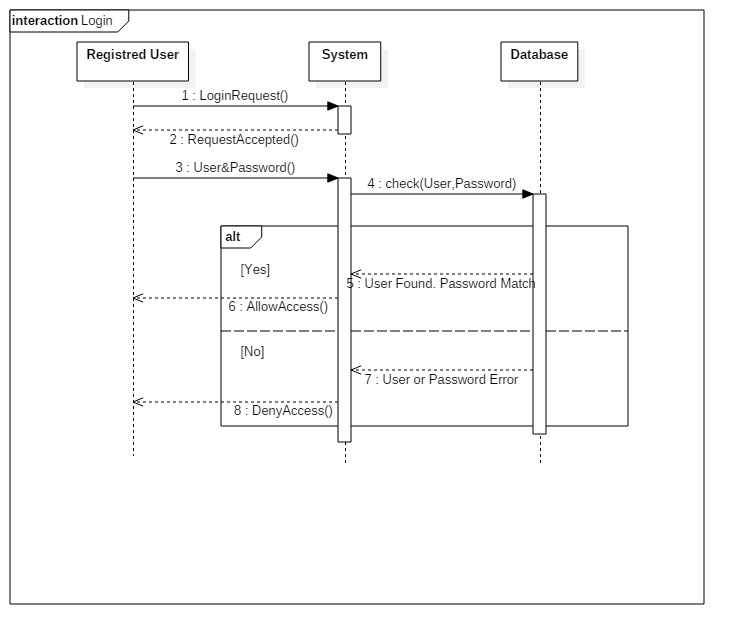
\includegraphics[width=6in]{./diagrams/SequenceLogin.png}
	\caption{Sequence Diagram: Login}
	\label{fig:SequenceLogin}
\end{figure}

\subsection*{Create Meeting}
\begin{center}

	\begin{tabular}{|c||p{0.6\textwidth}|}
		\hline
		Name & Create appointment \\ \hline
		Actors & User \\ \hline
		Assumption & The user need to insert a new appointment in his personal calendar \\ \hline
		Pre-Conditions & \begin{itemize}
			\item The user has successfully signed to the system
			\item The user has already opened the window with the insertion form.
		\end{itemize} \\ \hline
		Flow of events & \begin{enumerate}
			\item The user creates a new appointment by inserting all the information needed in order to adding a new event correctly in his own calendar.
			\item The system check into the calendar if the location of the appointment is reachable in the allotted time or if the event is overlapping with other appointment.
			\item The user is informed by a warning message about the actual validation of the appointment.
			\item The user have to confirm o reject the insertion of the appointment
		\end{enumerate} \\ \hline
		Post-Conditions & The appointment of the user has been stored to the system in the event that he has confirmed the inclusion. \\ \hline
		Exception & An internal system error makes impossible to store the reservation data. The user is notified of the error \\ \hline		
	\end{tabular}
\end{center}

\begin{figure}[H]
	\centering
	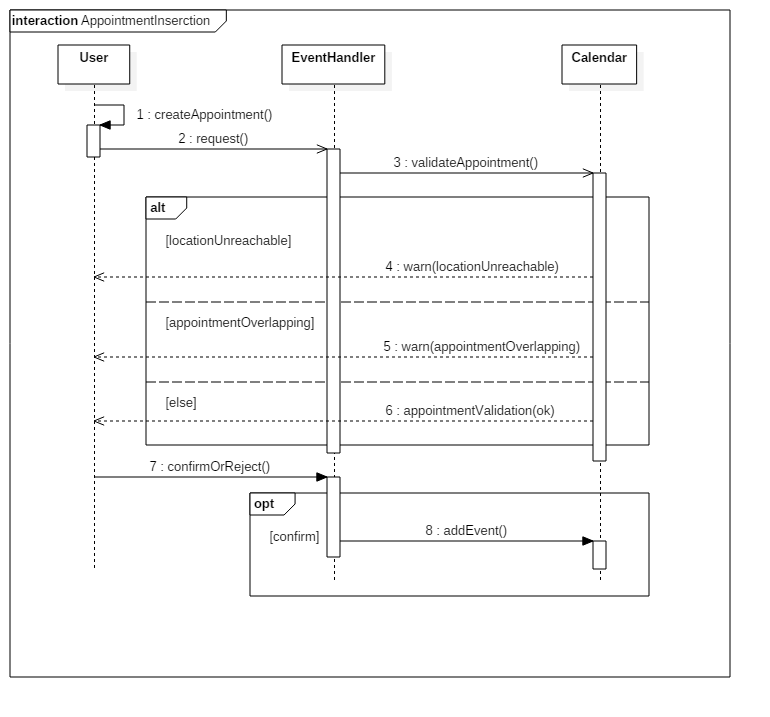
\includegraphics[width=6in]{./diagrams/AppointmentInserction.png}
	\caption{Sequence Diagram: Create Appointment}
	\label{fig:SequenceAddApp}
\end{figure}

[TODO] Mockups to be transferred when the use will be finished.

\begin{figure}[H]
	\caption{Main application landing}
	\centerline{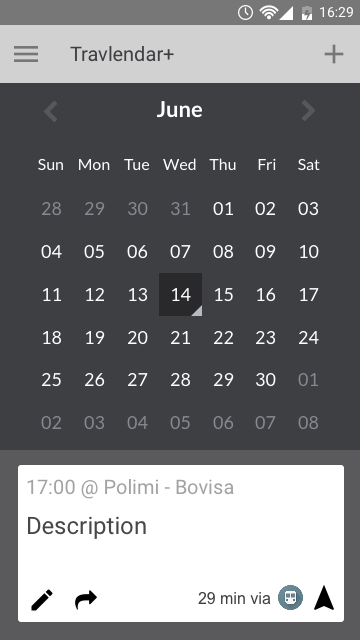
\psfig{file=images/home.png,width=0.6\textwidth} } 
\end{figure}
\begin{figure}[H]
	\caption{Menu view}
	\centerline{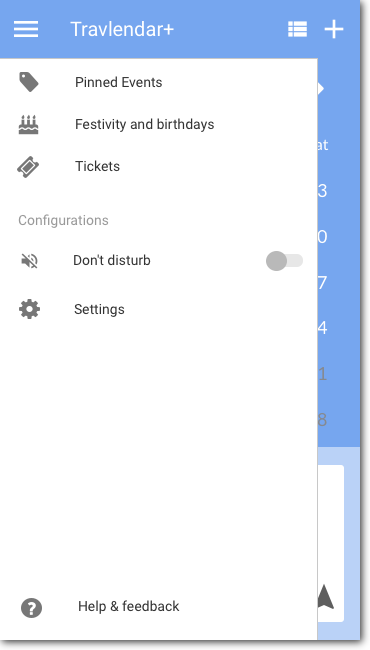
\psfig{file=images/menu.png,width=0.6\textwidth} }
\end{figure}
\begin{figure}[H]
	\caption{Create a new appointment}
	\centerline{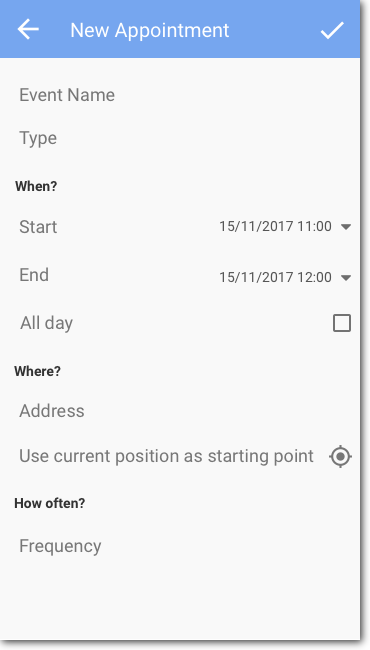
\psfig{file=images/appointment.png,width=0.6\textwidth} }
\end{figure}
\begin{figure}[H]
	\caption{Listing view of the appointments}
	\centerline{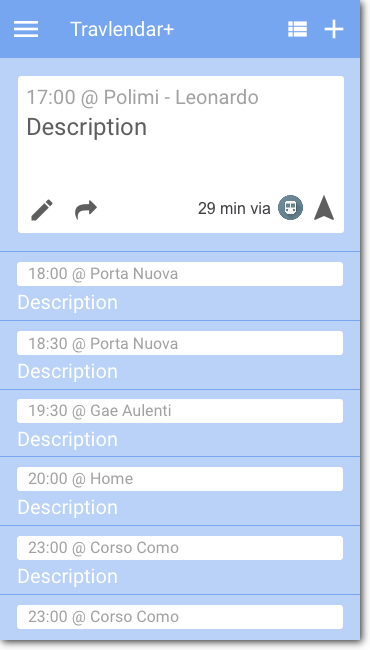
\psfig{file=images/listing.png,width=0.6\textwidth} }
\end{figure}
\begin{figure}[H]
	\caption{Notification from the application}
	\centerline{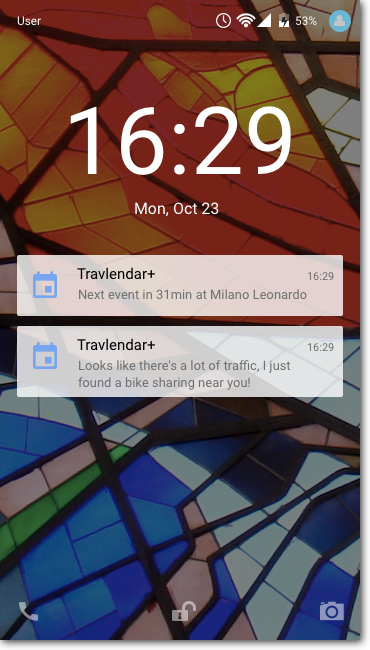
\psfig{file=images/lockscreen.png,width=0.6\textwidth} }
\end{figure}
\begin{figure}[H]
	\caption{Login}
	\centerline{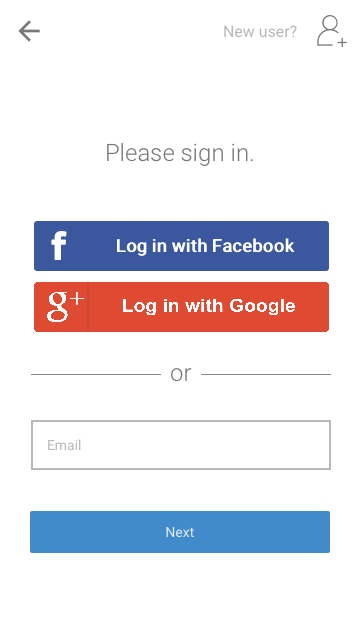
\psfig{file=images/login.png,width=0.6\textwidth} }
\end{figure}
\begin{figure}[H]
	\caption{Navigation with car}
	\centerline{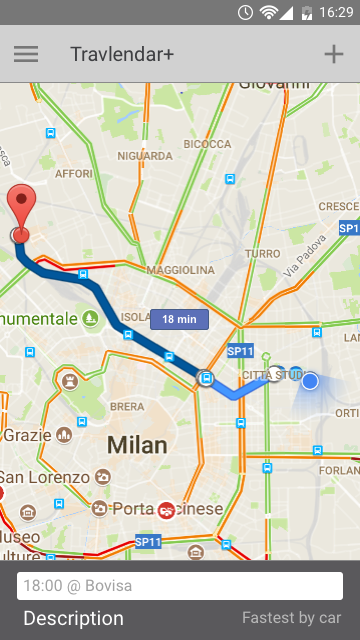
\psfig{file=images/map_car.png,width=0.6\textwidth} }
\end{figure}
\begin{figure}[H]
	\caption{Navigation with public transport}
	\centerline{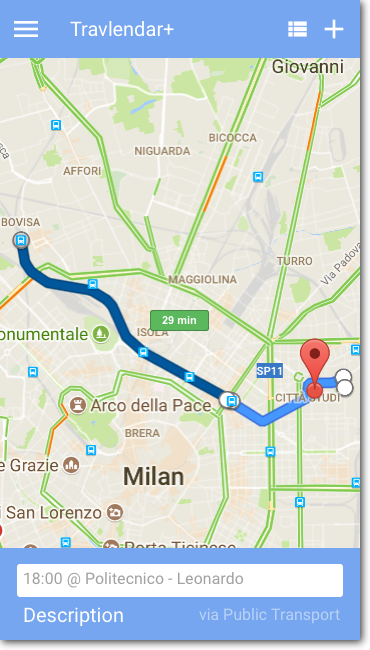
\psfig{file=images/map_pt.png,width=0.6\textwidth} }
\end{figure}
\begin{figure}[H]
	\caption{Settings}
	\centerline{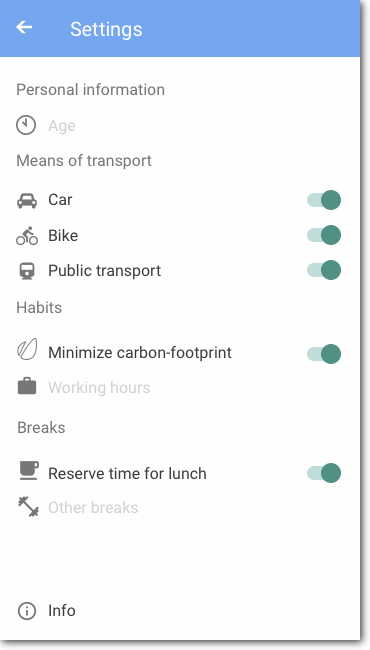
\psfig{file=images/settings.png,width=0.6\textwidth} }
\end{figure}

\section{Performance Requirements}
\label{sec:perf_req}
The user experience across the application should be fluid and with zero waiting time moving between the sections. Besides, there are a number of requirements that implies third party information retrieved through asynchronous requests so, the previous requirement can allow some tolerance.

\begin{enumerate}
\item There is no limit to the number of users registered to the application.
\item There is no limit to the number of the simultaneous users of the application.
\item The login process must be completed in less than 5 seconds once submitted the data.
\item The date text fields have to validate dates in real time.
\item The application going back to foreground has to be in the same state as when it was going to background
\end{enumerate}


\section{Design Constraints}
\label{sec:design_constraints}

\subsection{Standards compliance}
The application will be developed with the MVVM architectural pattern to allow the unification of the business logic and the coherence across all the various implementations.
The implementation on iOS and Android will be compliant with the App Store Review guidelines and Android Compatibility Definition Document.

\subsection{Hardware limitations}
The application relies on the usage of the GPS location and Internet access. In any case of disabled GPS or energy-saver option that blocks the retrieval of the User’s location or in case of no connectivity the application will not provide the user the ETA or the route navigation to reach an event nor the login function if the user is logged out.
\subsection{Any other constraint}
\input{requirements/other.tex}

\section{Software System Attributes}
\label{sec:sys_attribs}

\subsection{Reliability}
The application should have a 100 \% uptime in every designed scenario. Since the application relies on other systems API’s there will be the possibility to accept small variations in this requirement.
\subsection{Availability}
Regarding the mobile implementations the application will be available in the App Store and Play Store, instead, the desktop implementation will be available through the web app.
\subsection{Security}
The applications will perform every request in HTTPS to preserve the security of the user. 
Data that have to be stored in the device, will be encrypted with third-party libraries to avoid leakage of the user’s information.

\subsection{Maintainability}
The implementations will be developed with the MVVM architectural pattern allowing a modular integration of future new features or changes in the requirements. 
The application will rely on Google Maps API in order to maintain its core functionalities and not on other third-party libraries that could be deprecated in future OS versions.

\subsection{Portability}

\input{requirements/portability.tex}
